\chapter{\sffamily Centralised exchanges}

{\bfseries\sffamily Concept.} To define and develop an archetype simulation environment for centralised exchanges. In our classification scheme, this archetype is defined by a bidirectional star state partition graph topology and would make sense for simulations of financial, betting and housing markets as well as other forms of resource exchange. We will also discuss the typical ways in which the state partitions of the system may only partially be observed in realistic examples, and analyse how best to deal with each situation. For the mathematically-inclined, this chapter will define the mapping of our formalism to centralised exchanges. For the programmers, the software which is designed and described in this chapter can be found in the public Git respository here: \href{https://github.com/worldsoop/worldsoop}{https://github.com/worldsoop/worldsoop}.

\begin{figure}[h]
\centering
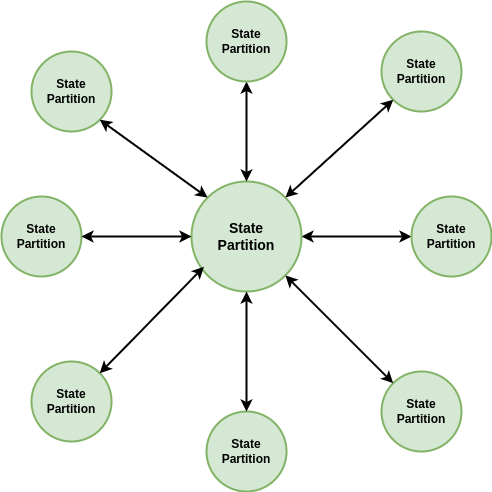
\includegraphics[width=9cm]{images/chapter-10-state-partition-graph.drawio.png}
\caption{State partition graph topology for centralised exchange archetypes.}
\label{fig:state-partition-graph-centralised-exchanges}
\end{figure}

\textcolor{red}{
\begin{itemize}
\item{Talk about data}
\item{Financial market RL papers}
\item{Betting market RL papers}
\item{Housing market policy control papers}
\item{(Biological?) Resource exchange control papers} 
\end{itemize}
}

